\documentclass[tikz, border=10pt]{standalone}
\usepackage{tikz}
\usepackage[utf8]{inputenc}

\definecolor{garnet}{HTML}{73000A}
\definecolor{atlantic}{HTML}{466A9F}
\definecolor{rose}{HTML}{CC2E40}
\definecolor{warmgrey}{HTML}{676156}
\definecolor{bk70}{HTML}{5C5C5C}

\begin{document}
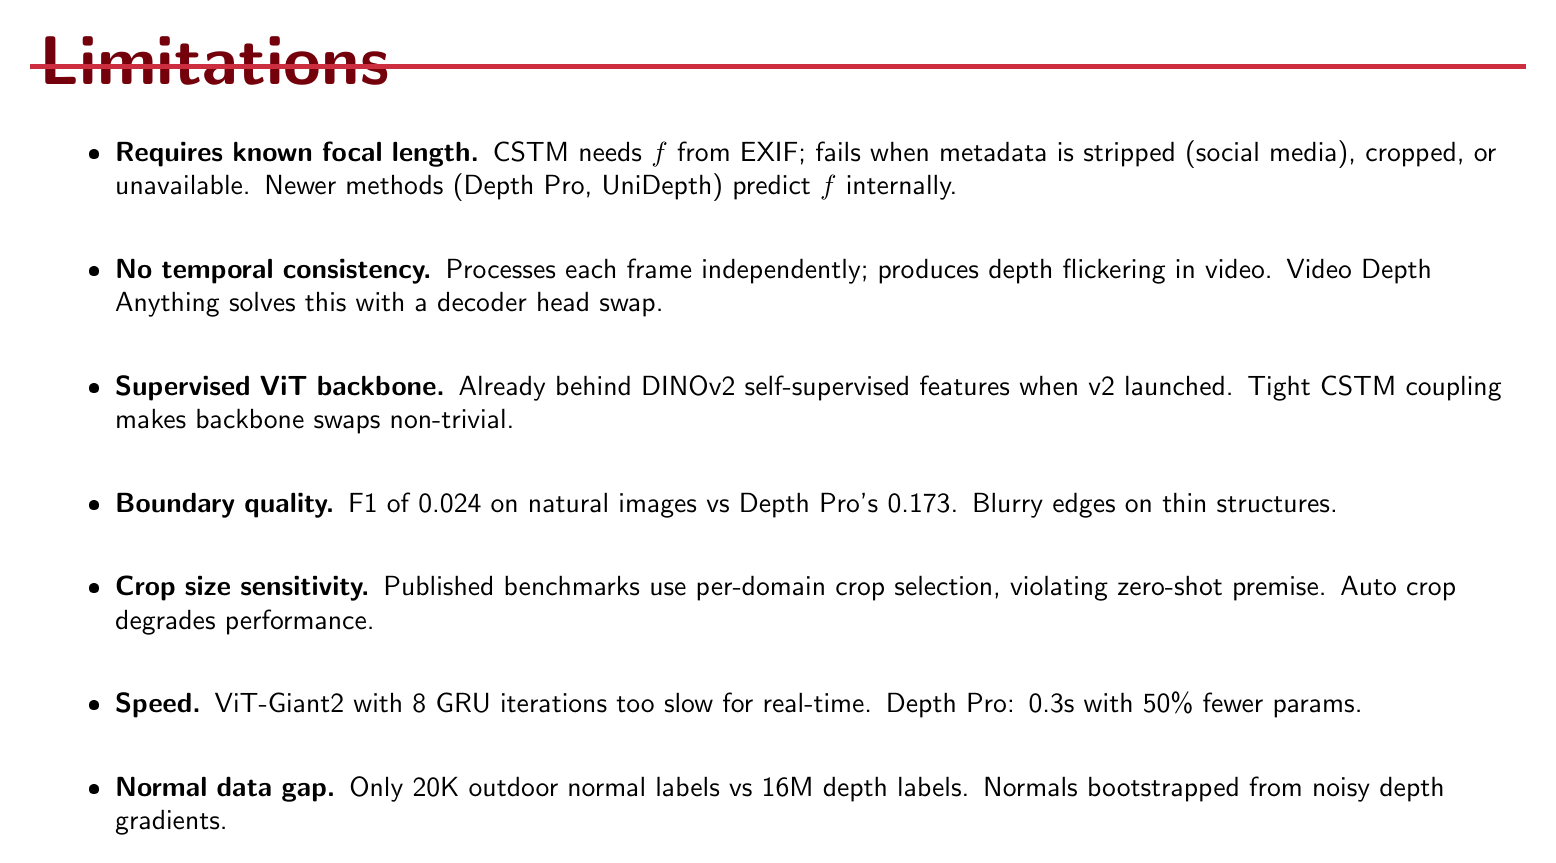
\begin{tikzpicture}[x=1cm, y=1cm]

  % Title
  \node[anchor=north west, font=\sffamily\bfseries\fontsize{36}{40}\selectfont, text=garnet]
    at (0.5, 23.5) {Limitations};

  % Horizontal line under title
  \draw[line width=1.5pt, color=rose] (0.5, 23) -- (19.5, 23);

  % Content area with itemized list
  \node[anchor=north west, text width=18.5cm, inner sep=0]
    at (0.7, 22.5) {
      \sffamily\fontsize{10}{12}\selectfont
      \begin{itemize}
        \itemsep=0.5cm
        \item \textbf{Requires known focal length.} CSTM needs $f$ from EXIF; fails when metadata is stripped (social media), cropped, or unavailable. Newer methods (Depth Pro, UniDepth) predict $f$ internally.

        \item \textbf{No temporal consistency.} Processes each frame independently; produces depth flickering in video. Video Depth Anything solves this with a decoder head swap.

        \item \textbf{Supervised ViT backbone.} Already behind DINOv2 self-supervised features when v2 launched. Tight CSTM coupling makes backbone swaps non-trivial.

        \item \textbf{Boundary quality.} F1 of 0.024 on natural images vs Depth Pro's 0.173. Blurry edges on thin structures.

        \item \textbf{Crop size sensitivity.} Published benchmarks use per-domain crop selection, violating zero-shot premise. Auto crop degrades performance.

        \item \textbf{Speed.} ViT-Giant2 with 8 GRU iterations too slow for real-time. Depth Pro: 0.3s with 50\% fewer params.

        \item \textbf{Normal data gap.} Only 20K outdoor normal labels vs 16M depth labels. Normals bootstrapped from noisy depth gradients.
      \end{itemize}
    };

\end{tikzpicture}
\end{document}
